\section{Functions}
Functions are like machines that take some input and produce some output. In the case of mathematical functions, these inputs and outputs are usually numbers. There are more general notions, taking other types of inputs and producing other types of output, for example sets, vectors, matrices, etc. but here, we will mainly look at functions that take one number as input and produce another number as output and those two numbers will typically assumed to be real numbers. The output of a function is supposed to depend only on the input and will be uniquely defined in the sense that if you apply the same input to a function multiple times, you will always get the same output. The role of the function is to "map" the input value to its corresponding output value. That's why functions are also sometimes called maps.

% That notion of a function is different from the notion of a function in imperative programming where the output of functions can depend on all sorts of internal and external state.

% Functions may also be called "maps":
% https://en.wikipedia.org/wiki/Map_(mathematics)

%===================================================================================================
\subsection{Domain and Range}
The two sets (of numbers) from which inputs can be taken and outputs will be produced are called the \emph{domain} and \emph{range} of the function respectively. Functions are usually denoted by lowercase letters such as $f,g,h$ etc. If a function takes real numbers as inputs and also produces real numbers as output, we write this as: $f: \mathbb{R} \rightarrow \mathbb{R}$. The argument of the function is usually denoted by $x$ and and is written in parentheses and the output is often denoted by $y$. When we write something like $y = f(x)$, we mean that the function $f$ produces the number $y$ as output when we give it the number $x$ as input. An example could be $y = f(x) = x^2$. The function would just square the input and return that as result. 

%\medskip
\subsubsection{Codomain and Image}
There is a little ambiguity with respect to the notion of range. It may mean either one these two things: sometimes it may mean the set of numbers from which outputs can \emph{potentially} be drawn and sometimes the (possibly smaller) set of numbers, that can \emph{actually} be the result. For example, if the domain of $f(x) = x^2$, is taken to be the set real numbers $\mathbb{R}$, we could think of $f$ as a mapping between real numbers and real numbers, i.e. $f: \mathbb{R} \rightarrow \mathbb{R}$. However, not all possible real numbers are reached because the result of $x^2$ will never be a negative number. We could also consider $f$ as a function from the real numbers to the \emph{nonnegative} real numbers, i.e. $f: \mathbb{R} \rightarrow \mathbb{R}^+_0$. To distinguish these two notions, sometimes the term "codomain" is used for the set that outputs could potentially be drawn from and "image" is used for the set from which numbers are actually produced by the function for a given input domain. You may also find authors talk about the image of a set under a function $f$ where that set is a subset of the domain of $f$. By this, they mean the set of output values that a function produces for the given set of input values. For example, the image of the interval $[3,5)$ under $f(x) = x^2$ is the interval $[9,25)$. The converse of this is called the \emph{pre-image} which is the set of input values that gives rise to a given set of output values. The pre-image of $[9,25)$ under $f(x) = x^2$ is $[3,5) \cup (-5,-3]$, for example. You may sometimes see expressions where a set $A$ is given as an argument to a function $f$, denoted as $f(A)$ or $f[A]$. What is meant by that is the image of the set $A$ under $f$ which is again a set. For the pre-image of a set $B$, you may see notations like $f^{-1}(B)$ or  $f^{-1}[B]$. The bracket notation is actually preferable because it makes clear that a set is taken as input rather than a single (numeric) argument. However, most authors tend to use the more sloppy parentheses notation for both - single arguments and sets of arguments. This may lead to confusion in certain cases. These cases may seem contrived to the beginner but they actually may occur in practice in more advanced math contexts, so we will adopt the bracket notation here.


% https://www.youtube.com/watch?v=3czgfHULZCs
% 1:56:48: injective = into, surjective = onto ...but that sounds questionable

% https://en.wikipedia.org/wiki/Domain_of_a_function
% https://en.wikipedia.org/wiki/Range_of_a_function

% If a set is given as input to a function to produce the image set A, it is better to use bracket rather than parentheses notation, i.e f[A] rather than f(A) (Weitz explains in one of his videos why - it's in the 2023 course, the videoo about function, I think.). Here:
% https://www.youtube.com/watch?v=1DK_5koM-1o&list=PLb0zKSynM2PCLnXVwfjVcefXa6iZA-an4&index=20
% the relevant part starts at around 7:30, 14:58
% Maybe elaborate this a bit

% The codomain "contains" the set of outputs
% https://www.youtube.com/watch?v=szfsGJ_PGQ0

%===================================================================================================
\subsection{Taxonomy}
There are certain features that a function may or may not have which turn out to be important for classification. A function is said to be \emph{monotonically increasing}, if from $a \geq b$ follows $f(a) \geq f(b)$. It means that the function either goes upward or stays constant but never goes downward. If the stronger condition  $a > b \Rightarrow f(a) > f(b)$ holds true, then $f$ is \emph{strictly monotonically increasing}. Such a function really goes upward everywhere. Not even plateaus are allowed. A \emph{(strictly) monotonically decreasing} function is defined analogously with $\leq, <$ rather than $\geq, >$. If a function is either (strictly) monotonically increasing or decreasing, it is called \emph{(strictly) monotonic}. A function $f$ is said to be \emph{bounded from above} when there is some finite number $U$ such that $f(x) \leq U$ for all $x$. The number $U$ is called an \emph{upper bound} for $f$. Likewise, a function $f$ is called bounded from below, when there's some number $L$ such that $f(x) \geq L$ for all $x$. In this case, $L$ is called a \emph{lower bound} for $f$. A function that is bounded from below and above is called \emph{bounded}. A function for which we have $f(x) = f(-x)$ has \emph{even symmetry} and a function with $f(x) = -f(-x)$ has \emph{odd symmetry}. Every function $f$ can be decomposed into an even part $f_e$ and odd part $f_o$ like so: 
\begin{equation}
\label{Eq:EvenOddFuncDecomp}
f_e(x) = \frac{f(x) + f(-x)}{2}, \;\;
f_o(x) = \frac{f(x) - f(-x)}{2}, \qquad
f(x) = f_e(x) + f_o(x)
\end{equation}
\emph{Injectivity}, \emph{surjectivity} and \emph{bijectivity} are also important features which have already been discussed in the section about set theory. To reiterate, injectivity means that different inputs get mapped to different outputs: $x_1 \neq x_2 \Rightarrow f(x_1) \neq f(x_2)$. This is sometimes also called a \emph{one-to-one} mapping. Surjectivity means that all possible numbers from the codomain are reached: $\forall y \exists x: f(x) = y$. A surjective function is sometimes also called \emph{onto} - it maps them domain onto the full codomain. Bijectivity means injectivity and surjectivity, i.e. the function is one-to-one and onto. Bijective functions are \emph{invertible}. Functions can also be \emph{periodic}. That means that there exists some number $p$, called the period, such that $f(x) = f(x + k p)$ for all inputs $x$ and all integers $k$. Such a function repeats itself over and over. Functions may have \emph{asymptotes} which are straight lines which the function approaches as the argument goes to plus or minus infinity. Asymptotes can also be vertical lines. In this case, the line is approached as the argument approaches a finite value and at that value itself, the function is usually undefined. When a function $f(x)$ has a vertical asymptote at some input value $x_0$, we call $x_0$ a \emph{pole} of the function. A function is said to be \emph{compactly supported}, if it is nonzero only in some finite interval and zero outside that interval. A function is called \emph{convex} if you can pick any two points $(a,f(a)),(b,f(b))$ on its graph, connect them with a straight line and the function will be below that line everywhere. The function behaves like a chain hanging down, i.e. it is curved downward like a bowl. The opposite of convex is \emph{concave}. Such functions are everywhere above the straight line. They look like an arch. A \emph{continuous} function is one that can be drawn without lifting the pencil or drawing vertical lines. Functions can also be classified according to their degree of \emph{smoothness} and/or according to whether or not they have a finite area under their graph. To define exactly what that means, we will need a few tools from calculus (differentiability, integrability), so we will defer further discussion about these features to later chapters.

% surjective: codomain coincides with image?

%===================================================================================================
\subsection{Defining a Function}

\paragraph{Explicit Rules}
One way to define a function is to prescribe a simple \emph{calculation rule} such as $f(x) = x^2 + 3 x - 5$ that applies equally to all possible inputs $x$. Up to until a few hundred years, this was the only way that was acceptable for mathematicians to define a function. Today, we have become a lot more liberal in that regard and allow functions to be defined in more esoteric ways. Some of these ways will involve concepts that are discussed only later in the book. If you don't understand these definitions, you can skip them on a first reading. In a first pass, you need to understand only this and the next way.

\paragraph{Piecewise Definitions}
A slightly more complicated way to define a function would be to have different calculation rules for different subsets of the domain. If these subsets are succesive intervals of the real number line, this way of defining a function is called a \emph{piecewise definition}. They are written down like this:
\begin{equation}
f(x) = 
\begin{cases} 
 0 \quad& x < 0 \\
 -x     & 0   \leq x < 1 \\
 x^2    & x \geq 1
\end{cases}
\end{equation}
This means, the function will output $0$ for $x < 0$ and $-x$ when $x$ is between zero and one (including zero, excluding one) and $x^2$ when $x \geq 1$. The example function is discontinuous at $x=1$. It jumps from $-1$ to $+1$ there. At zero, it has a corner - that is: a discontinuity in its slope.

% Maybe try to put a small plot next to the definition. There's enough space

\paragraph{Conditional Definitions}
The piecewise definition is a specific kind of a conditional definition where the conditions are of the form "if $x$ is in interval ... then ...". A function can also be defined by more general conditions such as:
\begin{equation}
f(x) = 
\begin{cases} 
 1 \quad& x \in    \mathbb{Q} \\
 0      & x \notin \mathbb{Q}
\end{cases}
\end{equation}
The function given above is called the Dirichlet function or indicator function of the rational numbers. It outputs one for rational inputs and zero for irrational inputs.

\paragraph{Definition by Data}
A function can also be defined by recorded data points of some measurement. To turn these discrete data points into a continuous function, one would also have to prescribe some sort of \emph{interpolation} rule such as "connect the dots by straight lines". The data together with the interpolation rule constitute a bona fide function: we can give it an input $x$ and it will give back an output $y$. 

\paragraph{Algorithmic}
Functions can be defined by the limit of some infinite recursive process or algorithm. An example of that is Bolzano's function. Such functions will often show self-similar, "fractal" behavior: you can zoom in as much as you like and it will always look similar. 
...TBC...ToDo: explain construction rule
% https://de.wikipedia.org/wiki/Bolzanofunktion
% https://demonstrations.wolfram.com/BolzanosFunction/
% Maybe "Algorithmic" is a too general term here. Maybe use "Recursive" or "Geometric". It's basically a recursively applied geometric construction rule. Maybe "Recursively Geometric". Or "as limit"

\paragraph{Infinite Sums}
The infinite process is sometimes defined to be an infinite sum. The individual terms are defined in terms of already known, simpler functions. An example of such a definition is the Weierstrass function defined as:
\begin{equation}
f(x) = \sum_{n=0}^\infty a^n \cos(b^n \pi x), 
\qquad 0 < a < 1, \; b \in \mathbb{N}, odd, b \geq 7
\end{equation}
It has two tweakable parameters $a,b$. It is defined as an infinite sum of exponentially weighted sinusoidal functions. This function has also a self-similar nature and a couple of strange properties that were unheard of in mathematics up to the 19th century such as being continuous everywhere but differentiable nowhere.
% https://en.wikipedia.org/wiki/Weierstrass_function

\paragraph{Power Series}
Often we will encounter infinite sums of weighted powers of $x$. A function definition based on such a sum is called a \emph{power series} definition. Most of our common functions can be expressed as such a power series even though they may have originally have been constructed by other ways. Exponential and sinusoidal functions are usually first defined by means of limiting processes or geometric constructions respectively. However, they do also have power series based definitions. They can be found from the original definitions by means of a Taylor expansion. This is a topic we will discuss in more detail in the calculus chapter. This process leads to:
\begin{equation}
e^x = \sum_{k=0}^\infty \frac{x^k}{k!}, \quad
\sin(x) = ...
\end{equation}
Power series are often used to expand the domain of a function - for example, from the real to the complex numbers. This works out so nicely because all that we need to evaluate a power series is to know, how to add or multiply two objects together and how to scale an object by a factor. When we have objects on which we have these 3 operations defined, we can evaluate, for example, the exponential function of that object via the above power series. The "object" can be a real or complex number - or it can be something else such as a matrix or an operator. We'll see later what these things are. Of course, such a power series does not need to originate from already known functions. It can be made up in any way you like - you just need to prescribe some rule to compute the weights. How you came up with that rule doesn't matter. What matters is the question, whether or not the series actually converges. More on that in the section about series in the calculus chapter.

\paragraph{Analytic Continuation}
Speaking of convergence, consider the following infinite sum:
\begin{equation}
	f(x) = \sum_{n=1}^\infty \frac{1}{n^x}
\end{equation}
This sum converges only for $x > 1$. If we allow complex arguments, the condition is $\Re(x) > 1$. So in the complex plane, this sum above defines a function for those complex numbers whose real part is greater than one. For other values, the function is as of yet undefined. However, as we will see later, complex analysis provides a tool known as \emph{analytic continuation} by means of which we can uniquely expand the domain of the function to the whole complex plane except for the single point $x=1$. The so defined function is known as the Riemann Zeta function and an important object in number theory due to its unexpected connection to prime numbers. The point that I want to make here is that the process of analytic continuation gives us yet another way to define a function.

\paragraph{Continued Fractions}
Another infinite process that is sometimes useful to define a function is called a \emph{continued fraction expansion}...TBC...

\paragraph{Inverse Functions}
A function can be defined by its inverse function. In general, you can take any given function $y = g(x)$ and then define another function $f$ by asking: "for a given $y$, what $x$ would I have to plug into my function $g$ to get that $y$?". For example, the logarithm can be defined to be the inverse of the exponential function. For a slightly more interesting example, consider the function $g(x) = x e^x$. Its inverse cannot be expressed in terms of common functions. Yet, it does have an inverse (with some caveats). The inverse function of $x e^x$ is called the "product logarithm" or "Lambert-W" function and has applications in the solution of equations where an unknown $x$ appears as base and as exponent or inside and outside of a logarithm.
% https://en.wikipedia.org/wiki/Lambert_W_function
% https://en.wikipedia.org/wiki/Lambert_W_function#Applications
% y = x e^x  <->  log(y) = log(x) + x
% https://www.desmos.com/calculator/s3gxvjbovr

% $f(y) = g^{-1}(y)$
%ToDo: arcsin, ...
%$ actually, the Lambert-W function is a case of an inverse function - in this case, the inverse of x e^x. maybe for implicit functions use y e^y = x + sin(x)

% W solves the ODE: y' = y / (x*(1+y)), see:
% https://www.youtube.com/watch?v=cMZ_blqKKZU

\paragraph{Implicit Equations}
Defining a function via its inverse is a special case of an implicit function definition. In a more general setting, we could have a bivariate function of the form $g(x,y) = 0$. In the case of the product logarithm function, we would have $x = y e^y$, so $g(x,y) = 0 = y e^y - x$.  This is an equation that can be solved for $x$ on one side of the equation. That's why we can define a function in terms of the inverse of the other side. But that doesn't always have to be the case. Consider modifying the equation $x = y e^y$ to $x + x^5 = y e^y$ or, equivalently $g(x,y) = 0 = y e^y - x - x^5$. Now, we can't  solve for a single $x$ on one side. And as before, we can't solve for $y$ either. Still, we can ask: "for a given $y$, what value of $x$ can I plug into $g(x,y)$ such that it evaluates to zero?" or "for a given $x$, what $y$ ...". There doesn't have to be a solution and if there is one, it doesn't need to be unique. But if there is a unique solution, then that equation defines a function. If there are multiple solutions, we may pick one of them to be our function of interest. You can play with the function defined by $ y e^y = x + b \sin(a x)$ a bit here on Desmos: \href{https://www.desmos.com/calculator/jfxwuhot8k}{jfxwuhot8k}. Tweak the parameters $a,b$. When any of them is zero, then the function is the regular product-log function. When both are nonzero, we get a wiggly version of it. ...TBC...


% \href{https://www.desmos.com/calculator/t3t92nihws}{t3t92nihws}

% https://en.wikipedia.org/wiki/Implicit_function

% y e^y = x + x^5
% https://www.desmos.com/calculator/ekao9wnrun
% https://www.desmos.com/calculator/t3t92nihws

% y e^y = x + b sin(a x)
% https://www.desmos.com/calculator/izay7xuihf
% https://www.desmos.com/calculator/jfxwuhot8k

% y + sin(y)   = x e^x      a wiggly version of Lambert-W
% y + sin(a y) = x e^x      wiggles get stronger for a > 1, it becomes multi-valued
% https://www.desmos.com/calculator/mowoqggdpj

% x tanh(x) = y atan(y)     has two graphs
% https://www.desmos.com/calculator/9cfsbbm0d9


%Now we want to cosider functions defined by so called \emph{implicit equations}. These are equations of the form $g(x,y) = 0$ for some given function bivariate $g$. They define a set of points in the $xy$-plane. Now, we can define a function $y(x)$ by requiring that it should satisfy our implicit equation, i.e. $g(x,y(x)) = 0$ is satisfied for all $x$ in some domain. That's an implicit definition for $y(x)$. For example, we could require the following equation to hold:
%\begin{equation}
% y e^y = x \;  \Leftrightarrow \; x - y e^y = 0 
%\end{equation}
%In this case $g(x,y) = x - y e^y$. I did not make up this example. The so defined function $y(x)$ is called the "Lambert-W" function or "product-logarithm" function. 

% Move that into the Interlude:


\paragraph{Interlude - Evaluation}
Of course, an implicit definition tells us nothing at all about how we would go about evaluating $y$ for a given $x$. Nonetheless, it is a valid definition. Definitions do not necessarily need to prescribe an explicit evaluation algorithm. They are supposed to tell us \emph{what} it is, not \emph{how} we may compute it. If they do tell us how to compute it, that's a bonus. There are algorithms to solve such implicit equations though. But that's a topic for a later chapter. You may also wonder how we are supposed to evaluate functions that are defined by some infinite process. The answer is: on a computer, we cannot really represent real numbers exactly anyway. Our usual floating point numbers are always approximations. They attempt to approximate the real numbers - but can do so only up to a finite precision. So, from a practical point of view, it is good enough to be able to evaluate functions up to some given precision. For the infinite processes, that usually means that we can obtain a sufficiently precise approximation of the function by only doing a finite number of steps until we deem the result to be close enough. The best we can expect is to be precise within one ulp ("unit in the last place"). Usually, we'll accept even much higher errors.





\paragraph{Functional Equations}
Now let's consider the factorial function $n! = 1 \cdot 2 \cdot 3 \cdot \ldots \cdot n$. As it stands, it's defined only for natural numbers. There is a way to define it for all real and even complex numbers. The key lies in the observation of the factorial's functional equation\footnote{A functional equation is an equation that relates values of a function at different evaluation points (VERIFY!). Here, it relates the values of the factorial function at the evaluation points $n$ and $n-1$.} which is given by $n! = n \cdot (n-1)!$. In our expanded definition, we want that equation to be satisfied for all real inputs. So we search for a continuous function $f(x)$ for which the functional equation $f(x) = x \cdot f(x-1)$ holds true. It can be shown that the following integral based definitions:
\begin{equation}
\Pi(x)    = \int_0^\infty t^x e^{-t} \, dt, \quad
\Gamma(x) = \Pi(x-1) = \int_0^\infty t^{x-1} e^{-t} \, dt,
\end{equation}
do indeed lead to functions that satisfy the desired functional equation. The first definition agrees with the factorials at the naturals, i.e. $\Pi(x) = x!$ for $x \in \mathbb{N}$. That means, it interpolates (i.e. makes continuous) the formerly discrete factorial function. The second definition is called the \emph{gamma function} and it agrees with the shifted factorial function. There is some discussion on \href{https://math.stackexchange.com/questions/1362523/why-is-the-gamma-function-off-by-1-from-the-factorial}{stackexchange} about why the gamma function might have been defined with that strange shift. Supposedly, it will make some higher level stuff more convenient but at first, it seems more unnatural and inconvenient than the $\Pi$ function. Nevertheless, it's the gamma function that is used in math all over the place. Anyway, my point here is that a function definition can be based on a functional equation. 
[VERIFY all of this!]

% Differentiating The FACTORIAL?! | Laid Back Math, Episode 20
% https://www.youtube.com/watch?v=gQKc308e-R4
% has good derivation for why gamma satisfies the functional equation of the factorial

\paragraph{Parameter Integrals}
In this case of the factorial function, the solution of the functional equation led to a definition in terms of a \emph{parameter integral} which is an integral in which the integrand depends on a parameter - here $x$.
I think, the general way to define a function $f$ in terms of a parameter integral is to have some function $g(x,t)$ and then use:
\begin{equation}
 f(x)  = \int_{a(x)}^{b(x)} g(t,x) \, dt
\end{equation}
For $\Pi(x)$ we have $g(x,t) = t^x e^{-x}, a(x) = 0, b(x) = \infty$.
[VERIFY all of this!]
...TBC...
% https://en.wikipedia.org/wiki/Gamma_function
% https://math.stackexchange.com/questions/1362523/why-is-the-gamma-function-off-by-1-from-the-factorial
% https://mathoverflow.net/questions/20960/why-is-the-gamma-function-shifted-from-the-factorial-by-1
% https://de.wikipedia.org/wiki/Parameterintegral
% Arens pg 409 ff, Bärwolff pg 166 (1 example),

\paragraph{Antiderivatives}
Speaking of integrals - we sometimes have a known function $f$ and want to define another function $F$ as an antiderivative of $f$. An important example is the area under a Gaussian bell curve from minus infinity up to some value $x$:
\begin{equation}
 F(x)  = \int_{-\infty}^{x} e^{-t^2}  \, dt
\end{equation}
I think, this can also be seen as another special case of a "parameter integral" definition with $g(x,t)=e^{-t^2}, a(x)= -\infty, b(x)=x$? ...figure out! Explain the erf-function

\paragraph{Differential Equations}
Finding an antiderivative is a problem of the form: for a given $g(x)$, find a function $f(x)$ such that $f'(x) = g(x)$. That equation is actually a special case of a more general class of equations called differential equations. These are equations in which the unknown function $f$ and derivatives of it may appear. A function $f$ that satisfies the differential equation is called a solution of the differential equation. Of course, saying something like: "let $f$ be the solution to the following differential equation..." is also a way of defining a function. There are some caveats, though: differential equations typically have many solutions so we need some additional constraints (typically boundary conditions or initial conditions) to pick out one of those solutions uniquely ...TBC...give examples for how exp and sin can be defined by an ODE, mention Bessel functions
%Having seen how function can be defined via integrals, the next step is consider functions that are defined by differential equations...TBC...

% differential equations - start with simple examples like exp, sin, cos, the give more complex examples like Bessel

\paragraph{Integral Equations}
An integral equation is an equation where an unknown function $f$ appears under an integral sign. Like with differential equations, solving the integral equation amounts to finding $f$. For example, imagine that we have two known functions $g, h$ and we want to find $f$ such that:
\begin{equation}
 \int_a^b f(u) h(x-u) \, du = g(x)
\end{equation}
for some constants $a,b$ (which are often minus and plus infinity). We could interpret $g$ as a recorded signal, $h$ as the impulse response or "kernel" of a filter and we want to reconstruct $f$ as it was before it went through the filter. The desired function $f$ appears under a convolution integral. This sort of equation is a particular kind of integral equation and does indeed define a function $f$.

%...TBC...
%ToDo: bring an example involving deconvolution - we are given a signal $g(x)$ which is supposed to be our desired $f(x)$ convolved with some known kernel $h(x)$. Then $f(x)$ appears under the convolution integral. Finding it involves deconvolution...can perhaps be done in the Foruier domain - but that's not the problem of the definition




%\paragraph{Implicit Differential Equations}
% well - so far we have said nothing in the paragraph about diffeqs that restricts us to explicit ones so we may consider the implicit ones to be already subsumed

%What about an implicit differential equation

% Yet another way to define a function:
% https://www.youtube.com/watch?v=U_5JDWR0HiM  Why care about infinite dimensions?
% it uses an (contraction) operator and defines the function as a fixed point of that operator. This coudl aczually be easily implemented numerically, I think.

\paragraph{Fixed Point of an Operator}
This is a fun one and rather exotic and requires some higher level math concepts, so feel free to skip it on a first read. An operator is a higher order function - an object that takes a function as input and returns another function as output. Such operators can have fixed points. These are functions for which the operator returns the input function unchanged - just like the function $f(x) = x^2$ has the fixed point $1$, i.e. returns one when plug in one. With such an operator in hand, we can define the function to be a fixed point of our given operator. 

% x^2 has the other fixed point x=0. x=0 is stable and x=1 is unstable, I think.

\paragraph{A Non Function}
Consider the following nonsensical looking attempt of defining a function:
\begin{equation}
f(x) = 
\begin{cases} 
0       \quad& x \neq 0 \\
\infty       & x = 0
\end{cases} \qquad \text{with} \qquad
\int_{-\infty}^{\infty} f(x) \, dx = 1
\end{equation}
We are trying to define a "function" that is zero everywhere except at zero. There, it should have an infinitely tall and infinitely thin spike. The (infinite) height of the spike should be adjusted in such a way that the total area under the function is unity. This "function" is called the Dirac delta function - and it isn't really a function at all because the definition does not really make sense formally. But when this strange function-like object appears under an integral, it suddenly starts to make a lot of sense and is very useful. We'll meet this bizarre Dirac spike again later in the chapter about functional analysis where it will be more rigorously defined as a \emph{distribution} which is a certain kind of \emph{functional}. Especially in physics and signal processing, we often work with this thing informally as if it were a function.


%ToDo: integral equation
% maybe make these subsubsection of an "Elementary functions"  section

\paragraph{Whoa!} That was a tour de force! I have presented quite a lot of ways how a mathematical function can be defined. Some of them required some rather high level math which doesn't really belong into such an early chapter. I did this to point out that the idea of "defining a function" can, when intepreted liberally as we do in the modern world, include much more diverse and creative ways rather than just a simple and explicit calculation rule. However - most functions that we encounter in everyday life are not of such a complicated nature. There's a set of functions that tends to pop up everywhere and constitutes a sort of basic mathematical vocabulary that everybody needs to be familiar with. I'm talking about the so called...

%===================================================================================================
\subsection{Elementary Functions}
In general, a function can be any mapping. But there is a certain set of functions that permeates mathematics so thoroughly that it has been given a special name: the elementary functions. These are all functions that can be constructed by a finite formula involving only the 4 basic arithmetic operations, roots, exponentials, logarithms, trigonometric functions and the inverses of all these functions.

% https://www.youtube.com/watch?v=l6w868U8C-M
% https://en.wikipedia.org/wiki/Elementary_function

%---------------------------------------------------------------------------------------------------
\subsubsection{Absolute Value aka Norm}
A simple but very important function is the \emph{absolute value} or \emph{norm} of some number $x$ which we commonly write as $|x|$ and read as "absolute value of $x$" or in some contexts also "norm of $x$". The former term applies to real numbers $x$ and the latter term applies in cases where $x$ is a more complicated object than a real number. Yes - that means the absolute value (or norm) function will later be generalized to more complicated objects (complex numbers, vectors, matrices, etc.) and by doing so, it will retain some of its important properties and that's perhaps the chief reason why it is such an important function despite being so humble. For a real number $x$, it can be defined as:
\begin{equation}
 |x| = \sqrt{x \cdot \overline{x}} = 
\begin{cases} 
  x \quad & \text{iff } x \geq 0 \\
 -x \quad & \text{iff } x   <  0 \\
\end{cases} 
\end{equation}
The piecewise definition on the right hand side is how we usually think of $|x|$ when $x$ is a real number. The definition with the square-root in the middle can at this point be taken as a provision for later generalizations and you don't need to worry about this right now, if it doesn't make any sense yet (spoiler: the overline will be used for complex conjugation and the product will generalize to a so called scalar product). Our absolute value function satisfies the following conditions for all $x,y \in \mathbb{R}$:

\medskip
\begin{tabular}{l l}
\label{Tab:Norm}
Non-negative:         & $|x| \geq 0$  \\
Positive definite:    & $|x| = 0 \Leftrightarrow x = 0$  \\
Multiplicative:       & $|x \cdot y| = |x| \cdot |y| $  \\
Triangle inequality:  & $|x + y| \leq |x| + |y| $
\end{tabular}
\medskip
%https://en.wikipedia.org/wiki/Norm_(mathematics)
% Die rationalen Zahlen liegen dicht (wie feiner Staub) in der Menge der reellen Zahlen
% https://www.youtube.com/watch?v=lWTf_Isveso
% I think, the non-negative property is already included in "positive definite". Maybe state it as:
% Positive definite:    & $|x| \geq 0,  |x| = 0 \Leftrightarrow x = 0$  \\

The idea of a norm function is that it should somehow measure the "size" of the object that it is being applied to. The first two conditions say that a norm can never be negative and it is zero if and only if the input is itself already zero. These conditions do indeed sound like some minimum requirements that we expect such a "norm" function to have if it should be interpretable as a size. Multiplicativity and triangle inequality are less obvious. The latter basically means that a direct path is always shorter than a roundabout path. We'll say more about this when we will meet vectors. These four are the properties that all functions shall have if they want to deserve to qualify for calling them a "norm" even when $x$ and $y$ can later be more complicated objects than real numbers. Some more properties immediately follow from these: $|x/y| = |x|/|y|$, $|x-y| = |x| + |y|$, $\bigl| (|x|-|y|) \bigr| \leq |x \pm y|$. In programming languages, the absolute value function is often called "abs". % and we may use that term as convenient abbreviation. 

\paragraph{The Signum Function}
A related function is the so called signum or sign function. It is the counterpart to the absolute value function in the sense that in contains precisely the information that was thrown away when applying the absolute value function - namely, the sign of the number. For real $x$, it is defined as:
\begin{equation}
\sign(x) = 
\begin{cases} 
 -1 \quad & \text{iff } x < 0 \\
  0 \quad & \text{iff } x = 0 \\ 
  1 \quad & \text{iff } x > 0 \\
\end{cases} 
\end{equation}
To reconstruct our original $x$, we can combine sign and norm: $x = \sign(x) \cdot |x|$. If we want to generalize that reconstruction property to more complex objects, we could define it via this relation: $\sign(x) = x / |x|$ (for $x \neq 0$). This is non-standard notation though and the term "sign" doesn't make sense if $x$ is not a real number. In the case where $x$ is a complex number or a vector, it would make more sense to call the quantity $x / |x|$ a "direction" which generalizes the idea of a "sign" (which can encode precisely two directions like "left" and "right" (and "none" as edge case for zero)).

\paragraph{Note}
I said formerly that an "elementary" function can only use the arithmetic operators, roots, the exponential and trig functions and the inverses of all of these. I didn't say anything about piecewise definitions, so one might reasonably question whether the absolute value and sign should qualify as "elementary". But the definition of the norm as $|x| = \sqrt{x^2}$ saves the day (in the reals, we have $\overline{x} = x$). Likewise, the (re)definition $\sign(x) = x / |x|$ saves the day for the sign function. We may need to make an exception for $x = 0$ though and maybe I'm being a bit sloppy here and maybe strictly speaking, the sign should not be listed in this category. But at least, it's certainly piecewise elementary.

% Zusammenhang zwischen normierten, metrischen und topologischen Räumen
% https://www.youtube.com/watch?v=3j8GIJd5-3A&list=PLHi0WgifODX19zsJhvCrizYEXiHY5qc9n


%---------------------------------------------------------------------------------------------------
%\subsubsection{Distance}



%---------------------------------------------------------------------------------------------------
\subsubsection{Complex Conjugation}

% -can be dragged out of sums and products
% -sqrt(z * conj(z)) = |z|

%---------------------------------------------------------------------------------------------------
\subsubsection{Polynomials}
A \emph{polynomial} can be written in various forms. Some important canonical forms are: (1) a weighted sum of integer powers of $x$, (2) a (scaled) product of so called linear factors, (3) a nested expression. So, a polynomial is a function that can be written in one of these forms\footnote{With some caveat: The given product form is guaranteed to exist only if we are assuming to work over the complex numbers (or some other algebraically closed field), which, for the time being, we indeed will assume. If we have only real numbers, there may be quadratic factors as well - and if we have only rational numbers or work over finite fields, we may have to include even higher degree factors.}:
\begin{equation}
 f(x) = \sum_{k=0}^n a_k x^k 
      = a_n \prod_{k=1}^{n} (x - r_k)
      = a_0 + x(a_1 + x(a_2 + \ldots + x(a_{n-1} + x a_n)))
\end{equation}
where the weights $a_k$ in the sum form are called the \emph{coefficients} of the polynomial and the highest power $n$ for which there is a nonzero coefficient is called the \emph{degree} of the polynomial and the coefficient $a_n$ in front of it is called the \emph{leading coefficient}. The $r_k$ in the product form are called the \emph{roots} of the polynomial. These are the values of $x$ where the output of the function $y = f(x)$ is zero. This is immediately obvious from the fact that a product is zero as soon as any of its factors is zero, which will clearly be the case if $x = r_k$ for one of the $r_k$. The roots $r_k$ may be real or complex and are not necessarily distinct. The number of times by which a root appears in the product is called the \emph{multiplicity} of the root. An important theorem, the \emph{fundamental theorem of algebra}, states that every polynomial of degree $n$ has exactly $n$ such roots in the complex plane (counted with multiplicity, i.e. a double root counts twice, etc.). You will sometimes find a weaker form of this statement called fundamental theorem of algebra, namely the statement that each polynomial of nonzero degree has a root. But the stronger statement immediately follows from the possibility of splitting off a linear factor and then recursively applying the same theorem to the other factor. It's usually preferable for a theorem to make the most precise and strongest possible statement from the weakest possible assumptions unless, perhaps, doing so would get in the way of comprehensibility. But that's not the case here so that's why I prefer the stronger version of the theorem that I stated first. By the way, the scaling factor $a_n$ in front of the product form is indeed the same $a_n$ as the $a_k, k=n$ coefficient in the sum form, i.e. the leading coefficient. Also, the $a_k$ in the nested form are the same coefficients as in the sum form. A polynomial of degree 1, i.e. a function of the form $f(x) = a_0 + a_1  x$, is a very simple special case which is of practical importance and is sometimes - somewhat inconsistently - called a linear function. This terminology is inconsistent because such a function satisfies the usual requirements for linearity - homogeneity and additivity - only when the additive constant is zero, i.e. when $a_0 = 0$. Nevertheless, you'll find that terminology used often, especially in high-school level math texts. That's because in these contexts, what they usually mean by "linear" is: "defines a line" rather than these more abstract homogeneity and additivity properties. In more advanced university-level texts, they may also be called \emph{affine} functions. In this context, "affine" usually means: "linear plus some offset". 

\paragraph{$\star$ Some Applications - Preview}
The practical importance of such affine functions is that we will often use them to approximate more complicated functions - a process known as \emph{linearization}\footnote{But shouldn't it then be called "affinization"? Math terminology is unfortunately not always totally consistent. I digress...}. This linearized function will have the same function value as the original function at some point of interest and will, moreover, also have the same slope (i.e. the same first derivative). A polynomial of degree 2, i.e. a function of the form $f(x) = a_0 + a_1 x + a_2 x^2$, is also called a quadratic polynomial. Such polynomials are often used to approximate an arbitrary function around a minimum or maximum in the context of \emph{optimization} problems. A linear approximation is not suitable in this case because the $a_1$ coefficient will be zero anyway so we need to go one degree higher if we don't just want a constant "approximation" (which doesn't really deserve this name - therefore the quotes). A quadratic approximation can also be used as a more accurate approximation than a linear one around arbitrary points and sometimes this is useful, too. And, of course, one can also use higher order polynomial approximations, as well. For some functions, when we approximate them with polynomials and crank up the degree, the approximations will actually converge to the original function. This happens, for example, in a \emph{Taylor expansion} or in \emph{Lagrange interpolation}. We'll look into the details of these applications later. Polynomials are generally used to do all sorts of approximations because polynomials are often much easier to deal with than other types of functions - especially when it comes to problems involving some calculus because polynomials are easy to integrate and differentiate in closed form. For example, if all you want is a numerical value for some definite integral over a function that is hard (or impossible) to integrate in closed form, you can take a (piecewise) polynomial approximation and integrate that instead and thereby obtain an approximation of your desired integral. This is done in \emph{numerical integration}. Generally, polynomials are used extensively in \emph{numerical analysis} which includes, besides numerical integration also \emph{numerical differentiation} and the numerical solution of (ordinary and partial) \emph{differential equations}. These things are all super important for applications in the natural sciences and in engineering. In data analysis and visualization, polynomials are also important for tasks like \emph{interpolation}, \emph{curve fitting}, etc.

%if your original function is hard to integrate in closed form, 

% "product form" = "linear factorization"

% quadratic approximations, biquads

\paragraph{Powers and Monomials}
The individual terms of the polynomial in its sum form, i.e. the $a_k x^k$ are called \emph{monomials}. If the coefficient $a_k$ is one, we are just dealing with a integer power of $x$ where the exponent is a natural number. There are some important rules for such natural powers of $x$:
\begin{equation}
\label{Eq:PowerRulesNatural}
x^n x^m = x^{n+m}, \qquad
\frac{x^n}{x^m} = x^{n-m}, \qquad
(x^n)^m =  x^{n m} =  (x^m)^n
\end{equation}
where the second rule, for the time being, makes only sense when $n-m$ is natural, i.e. $n \geq m$. We will see later that this restriction can be dropped, though. But for that, we need to \emph{define} what $x^a$ is supposed to mean when $a$ is not necessarily natural.
% ToDo: list power rules x^{n+m} = x^n x^m,  x^{n m} = (x^n)^m
% exlpain the term "monic"



\paragraph{Evaluation}
The evaluation of a polynomial is best done in nested form. This is the computationally most efficient way and also one of the most stable ways numerically\footnote{Numerical stability refers to the way in which small errors in the inputs affect the errors in the output - will errors tend to get amplified or not, etc.}. We assume that a polynomial of degree $n$ is represented in the computer as a list or array of $n+1$ coefficients $a_0, \ldots, a_n$.
\begin{lstlisting}
def polyEval(p, x):
	"""Evaluates the polynomial p at the given x using Horner's algorithm"""
	k = len(p)-1           # last valid index
	if(k < 0):
		return 0
	y = p[k]
	while(k > 0):
		k -= 1
		y = y*x + p[k]
	return y
\end{lstlisting}
This way of evaluating a polynomial is also known as Horner's rule.
...hmm...not sure, if code should appear in the normal text. maybe put it into an appendix? 


\paragraph{Addition and Subtraction}
Polynomials, given as arrays of coefficients, can be added and subtracted element wise. If the input arrays are of different length, i.e. the polynomials are of a different degree, the lower degree coefficient array has to be padded with zeros to match the length of the larger one.
%...python code is buggy

\paragraph{Multiplication}
When we multiply two polynomials $f(x), g(x)$ with degrees $m,n$ together, we will get a new polynomial of degree $m+n$. The coefficients of this new polynomial can be found by an algorithm called \emph{convolution}. Let's see how this would look like:
\begin{eqnarray}
&  (a_0 + a_1 x + a_2 x^2 + a_3 x^3 + \ldots)
   (b_0 + b_1 x + b_2 x^2 + b_3 x^3 + \ldots)  \\
=&  c_0 + c_1 x + c_2 x^2 + c_3 x^3 + c_4 x^4 + c_5 x^5 + c_6 x^6 + \ldots \\
=&  a_0 b_0 \\
&+ (a_0 b_1 + a_1 b_0) x \\
&+ (a_0 b_2 + a_1 b_1 + a_2 b_0) x^2 \\
&+ (a_0 b_3 + a_1 b_2 + a_2 b_1 + a_3 b_0) x^3  \\
&+ (a_0 b_4 + a_1 b_3 + a_2 b_2 + a_3 b_1 + a_4 b_0) x^4 \\
&+ (a_0 b_5 + a_1 b_4 + a_2 b_3 + a_3 b_2 + a_4 b_1 + a_5 b_0) x^5 \\
&+ (a_0 b_6 + a_1 b_5 + a_2 b_4 + a_3 b_3 + a_4 b_2 + a_5 b_1 + a_6 b_0) x^6 + \ldots
\end{eqnarray}
[TODO: suppress numbering for the individual lines] \newline
The coefficient $c_n$ in the resulting polynomial is the sum of all products of input coefficients $a_i, b_j$ such that $i+j = n$. Let's introduce another index $k$ to replace $i$ and then use $n-k$ to replace $j$. This ensures that $k + (n-k) = n$. We now have:
\begin{equation}
  c_n = \sum_{k=0}^n a_k b_{n-k}
\end{equation}
That formula to compute the new list of $c$-coefficients from the $a$- and $b$-coefficients is called convolution. Multiplication of two polynomials is achieved by convolving their coefficient lists (yes, the noun is \emph{convolution} and the verb is \emph{convolve} - not convolute). Convolution is an important mathematical operation that crops up in different variations everywhere. Polynomial multiplication is just one of the many places. Signal processing is full of it. Its continuous variant plays a role in the solution of certain differential equations which are all over the place in physics. You may have learned in high school how to do polynomial multiplication with pencil and paper and you have probably hated it just as much as your seatmate and everybody else including me. Don't worry - we don't do such things here. Instead, we teach a computer to do that boring calculation for us.

...TBC... TODo: give Python code for convolution - or give a reference to my C++ implementation
% \bigl(\sum_{n=0}^N  a_n x^n\bigr) \bigl( \sum_{k=0}^M b_k x^k \bigr) = $\sum_{n=0}^{N+M} c_n x^n, wher c_n = ...
% give a similar formula also for nesting and deconvolution

\paragraph{Division}
Let's now see, if we can reverse the process. Let's assume that we know the coefficient arrays $c_n$ and $b_n$ and want to figure out all the $a_n$. We need to make sure that the coefficients for like powers of $x$ match. For example, at the top of the triangle, we have the product $a_0 b_0$. That's how we computed the coeff for the constant term in the product polynomial $c_0$. So we have $c_0 = a_0 b_0$. That actually already tells us $a_0 = c_0 / b_0$. Now look at the line immediately below the tip of the triangle. The sum in brackets must equal $c_1$. But $c_1 = a_0 b_1 + a_1 b_0$ means $a_1 = (c_1 -a_0 b_1)/b_0$. We have found our next coefficient! Everything on the right is already known, The $b$- and $c$-coeffs are assumed to be known anyway and $a_0$ has just been computed in the previous step. One line more to establish the pattern: we must have $c_2 = a_0 b_2 + a_1 b_1 + a_2 b_0$ so we have $a_2 = (c_2 - a_0 b_2 - a_1 b_1)/b_0$. In general:
\begin{equation}
a_n = \frac{1}{b_0} (  c_n - \sum_{k=0}^{n-1} a_k b_{n-k} ) 
\end{equation}
[...but there's a caveat: what, if $b_0 = 0$? Maybe we should find $m$ as the index of the first nonzero $b$-coeff and use $b_m$ as divisor? I think, the upper limit of the sum can then be reduced to $n-m-1$. -> figure out! What about polynomial division with remainder? Maybe apply the deconv-algo to sequences $c_n, b_n$ where $c_n$ actually did \emph{not} arise from a product involving $b_n$? Point out the caveats and provide working code that takes care of them!]


%Oh my dog! Polynomial division! That pesky algorithm that we all once had to learn in school and then have forgotten for good! Worry not - you won't have to relearn it here and now. Executing algorithms with pencil and paper is not something we humans like to do and I personally find it as pointless as the next guy. Instead, I'll give you computer code for it, so we'll never ever have to do it again by hand. ....

% what if c = 1, b = 1 + x^2 - what a would we get by deconv? maybe some sort of polynomial approximation of 1 / (1 + x^2)? We get a0 = 1, a2 = -1, a4 = +1. I guess all odd coeffs are zero and the +-1 pattern for the even coeffs continues? Figure out! But it does indeed look like taking more such terms improves the approximation, see:
% https://www.desmos.com/calculator/7rekjnfmtw
% move this comment to the cpp code where we implement or test this deconv algo - make an experiment! Compare coeffs to Taylor coeffs and the Approximation to the Taylor approximation!

\paragraph{Composition}
We can also compose two polynomials in the sense that we take an input $x$, then first apply one polynomial $y = p(x)$ and to the result $y$, we then apply another polynomial $z = q(y) = q(p(x))$. The so defined function will be yet another polynomial. When $p$ has degree $m$ and $q$ has degree $n$, then the nested polynomial defined by $q(p(x))$ will have degree $m n$.

TODO: give algorithm for computing the coeffs of the nested polynomial in terms of coeffs of the two input polynomials

% degree is m n

%..tbc..
% product form, fundamental theorem of algebra, linear functions as special case
% factor out a linear factor, polynomial addition, multiplication, division - maybe with (pseudo) code or better: sage code, maybe provide als sage code for basic integer arithmetic - maybe in the section numbers in 

%\paragraph{$\star$ Companion Matrix}
% https://en.wikipedia.org/wiki/Companion_matrix
% https://en.wikipedia.org/wiki/Minimal_polynomial_(linear_algebra)


% Sturmsche Kette: Die exakte Anzahl der Nullstellen jedes Polynoms
% https://www.youtube.com/watch?v=gG7B1KQSg_I
% -Am Ende: Cauchy's Nullstelleninterval: Sei: M = 1 + max(a_0,a_1,..,a_{n-1}) / a_n. Dann liegen
%  die Nullstellen in [-M,M]

%---------------------------------------------------------------------------------------------------
\subsubsection{Rational Functions}
A rational function is a ratio or quotient of two polynomials, i.e. function of the form:
\begin{equation}
 f(x) = \frac{\sum_{k=0}^n a_k x^k}{\sum_{k=0}^m b_k x^k}
\end{equation}
Functions of that form...TBC...

% poles, zeros, cancellation

\paragraph{Partial Fraction Expansion}

% Maybe Polynomials and rational functions should get a section in their own right. Maybe after Linear Algebra...or maybe before it. Maybe is should be called "Polynomial Algebra" and be framed as another generalization of "Linear Algebra" where "Multilinear Algebra" is the other generalization. Polynomials do not necessarily need to be interpreted as functions - we can also interpret them as formal expressions. This interpretation can be generalized to non-convergent power series. The section should also consider multivariate polynomials. OK - it is now a section the Abstract Algebra chapter



%---------------------------------------------------------------------------------------------------
\subsubsection{Arbitrary Powers of $x$}
Polynomials are constructed as linear combinations (i.e. weighted sums) of nonnegative integer powers of the independent variable $x$. Surpassing the world of polynomials, we could also allow negative integer powers and identify the resulting functions as special cases of the rational functions. That is, it makes sense to define the function $f(x) = x^{-n}$ where $n > 0$ as the simple rational function $f(x) = \frac{1}{x^n}$. It can be verified that with such a definition, our rules given in (\ref{Eq:PowerRulesNatural}) continue to hold. This definition is an example of applying the \emph{principle of permanence} which says that, whenever we extend an existing definition to a larger domain, we should strive for doing it in such a way that our old rules continue to hold in this larger domain. Here, we extended the domain for allowed exponents from the natural to the integer numbers. Now we will generalize even more and look at what happens when we allow the exponent to be a rational, real or even complex number. That means, we are now interested in functions of the general form $f(x) = x^a$ where, $a$ is not restricted to a integer anymore. Let's start by investigating what $f(x) = x^{\frac{1}{n}}$ for positive natural $n$ could mean. The principle of permanence forces our hand to define this as $x^{\frac{1}{n}} = \sqrt[n]{x}$.

...TBC...

% https://en.wikipedia.org/wiki/Principle_of_permanence

% Use a^x = e^{x \ln (a)}, x^a = e^{a \ln (x)}

% Secret Kinks of Elementary Functions:
% https://www.youtube.com/watch?v=92wXQYcYLMg  
%
% What is the graph of x^a when a is not an integer? An unusual look at familiar functions #some2
% https://www.youtube.com/watch?v=_lb1AxwXLaM  






%---------------------------------------------------------------------------------------------------
\subsubsection{Algebraic Functions}
The set of algebraic functions contains all the functions that can be constructed from using the elementary operations and extracting roots....
% partial fraction expansion








%---------------------------------------------------------------------------------------------------
\subsubsection{Exponential Functions}
A general exponential function is a function of the form $y = f(x) = b^x$ for some constant $b$ which is called the basis (or base) in this context. Choosing Euler's number $\e = \lim_{n \rightarrow \infty} (1 + 1/n)^n = 2.71828\ldots$ as basis, we obtain \emph{the} exponential function $y = f(x) = \e^x = \exp(x)$. It can be defined via a power series, a limit or as inverse of a parameter integral [VERIFY the last]:
\begin{equation}
\e^x 
= \exp(x)
= \sum_{n=0}^{\infty} \frac{x^n}{n!}
= \lim_{n \rightarrow \infty} \left( 1 + \frac{x}{n} \right)^n, \quad
x = \int_1^y \frac{1}{t} \, dt
\end{equation}
% maybe replace the y in the parameter integral by e^x. I think, that is, what it means
% give continuous fraction expansion
It satisfies the following differential equation\footnote{Don't worry if you don't know what a differential equation is - we'll learn about them later and you can ignore it for now} and functional equation:
\begin{equation}
\frac{d}{dx} \e^x = \e^x, \quad
\e^{x+y} = \e^x \e^y
\end{equation}
This functional equation is pretty interesting indeed. It means that the exponential function translates between our two most important arithmetic operations addition and multiplication \footnote{subtraction and division are less important because they can be seen as mere inverses of the more fundamental operations of addition and multiplication}. The differential equation is quite noteworthy as well. It means that the exponential function is its own derivative. We can also insert complex arguments into the series definition. The resulting series will converge for any complex number $z$ whatsoever and the properties mentioned above continue to hold.

\medskip
In the complex domain, the exponential function also subsumes the - undeniably also very important - trigonometric functions sine and cosine that are so intimately related to the circle. All of these features are quite remarkable and secure the exponential function a top spot in the hall of fame of all functions in mathematics. It is even widely regarded as the most important function in all of mathematics and the chief reason for this is its functional equation, i.e. its ability to translate between addition and multiplication.



% Other properties:
% -it produces positive real output for real inputs
% -it never produces zero as output ...except for z = -inf - but this doesn't count because 
%  -inf is not a number?
% -for real x > 0, exp(x) > 1
% -exp(x) is strictly monotonically increasing on the real number line

[TODO: give formulas for change of basis, $(\e^x)^y = \e^{x y} = (\e^y)^x$, iff $xy = yx$, i.e. multiplications is commutative - which is true for complex numbers but may not be true in other number systems, explain how the exponential function can be generalized to other number systems using the power series, But: $(a^b)^c \neq a^{(b^c)}$ - exponentiation is not associative]

%As we will learn later, a   ...?...what did I want to write here?

% As we will learn later in functional analysis, it says that the exponential function is an eigenfunction of the derivative operator. 

% Verify:
% In terms of group theory, the exponential function $\e^x$ an isomorphism between the groups $(\mathbb{R}^+, +)$ and $(\mathbb{R}^+, \cdot)$. ..I think, all epxonential functions are such an isomorphism but the basis e is the only one with the special property that...what? It is its own derivative (without a scale factor)

% https://de.wikipedia.org/wiki/Exponentialfunktion
% https://en.wikipedia.org/wiki/Exponential_function

% https://en.wikipedia.org/wiki/E_(mathematical_constant)

% Make a paragraph about 0^0. List arguments for defining it as 0, as 1 or as undefined, see:
% https://www.youtube.com/watch?v=UW2VbHDnW5w
% https://www.youtube.com/watch?v=jNhjB4UfR9A
% https://www.youtube.com/watch?v=O8aKKKdQmxY


% Die wichtigste Funktion der gesamten Mathematik
% https://www.youtube.com/watch?v=zWBQXzjj5fY

% Permanenzprinzip:
% Rechenregeln sollen weiterhin gelten bei asuweitung des Definitionsbereichs

% https://www.youtube.com/watch?v=lXYxZBSkKLU
% Euler's number
% e   = lim n -> oo (1 + 1/n)^n
% 1/e = lim n -> oo (1 - 1/n)^n
% e   = sum_n  1/n!
% Maybe note that all definitions of e involve calculus operations. We could also evaluate the
% exp function at 1. This function itself is also defined via calc: there's this integral definition
% and the definition via the derivative
% https://www.spektrum.de/kolumne/wie-wurde-die-eulersche-zahl-entdeckt/2221156

% Die schönste Formel der Mathematik, die Kreiszahl Pi und die trigonometrischen Funktionen
% https://www.youtube.com/watch?v=-PYEguPdwdk
% 7:37  conj(e^z) = e^conj(z)


% Maybe motivate the power series expansion through Taylor series - but that requires calculus - maybe do it in the section about Taylor series. Motivate it from trying to approximate a function and a certain number of its derivatives at a point





%---------------------------------------------------------------------------------------------------
\subsubsection{Hyperbolic Functions}
When we decompose the exponential function into its odd and even parts, we obtain the so called \emph{hyperbolic sine} and \emph{hyperbolic cosine} functions $\sinh(x), \cosh(x)$:
\begin{equation}
\sinh(x) =	\frac{\e^x - \e^{-x}}{2}, \quad	
\cosh(x) =	\frac{\e^x + \e^{-x}}{2}, \quad
\end{equation}
By applying these odd/even decomposition formulas to the power series of $\e^x$ and simplify using the symmetries of $x^n$, we obtain the power series of $\sinh$ and $\cosh$: 
\begin{equation}
\sinh(x) = \sum_{n=0}^{\infty} \frac{x^{2n+1}}{(2n+1)!}, \qquad
\cosh(x) = \sum_{n=0}^{\infty} \frac{x^{2n}  }{(2n)!}
\end{equation}
These power series can also be constructed from the power series of the exponential function by just extracting the terms with odd exponents for $\sinh$ and the terms with even exponents for $\cosh$. This way of extracting the even and odd parts of a power series works for any function [VERIFY!]. The two functions satisfy the following system of coupled differential equations:
\begin{equation}
\frac{d}{dx} \sinh(x) = \cosh(x), \quad
\frac{d}{dx} \cosh(x) = \sinh(x)
\end{equation} 
If you repeatedly differentiate, you'll always cycle through the same two functions. So we have a 2-cycle here. As an interesting parallel, recall that the exponential function is its own derivative which can be viewed as a 1-cycle. There is also a pair of formulas for hyperbolic functions that parallels the functional equation of the exponential function:
\begin{equation}
\sinh(x+y) = \sinh(x) \cosh(y) + \cosh(x) \sinh(y), \quad
\cosh(x+y) = \cosh(x) \cosh(y) - \sinh(x) \sinh(y)
\end{equation}


%...TBC...give functional and differential equations




% Everything still makes sense when the argument is a complex number. 

%and when we form their quotient, we obtain the hyperbolic tangent $\tanh(x)$:
%\begin{equation}
%\tanh(x) =	\frac{\sinh(x)}{\cosh(x)} 
%         = \frac{\e^x - \e^{-x}}{\e^x + \e^{-x}}
%\end{equation}



% https://en.wikipedia.org/wiki/Hyperbolic_functions

% ToDo: maybe remove the tanh function from the eq above - introduce it later. maybe together with other functions like tan, sec, sech, cosec, etc..


%---------------------------------------------------------------------------------------------------
\subsubsection{Trigonometric Functions}
The trigonometric functions $\sin(x), \cos(x)$ originally arise from certain geometric considerations about triangles (more on that later in the geometry chapter) but, surprisingly, they can also be introduced in an entirely different way. I mentioned that the exponential function can be evaluated in the whole complex plane via its power series definition. If we evaluate it along the real number line, we get strictly monotonically increasing real values as outputs. Let's now evaluate the same power series along the imaginary line. That means, we pick a real number $x$ and look at the function $\e^{\i x}$. When we do that and separate the real and imaginary parts, we will arrive at:
\begin{equation}
\e^{\i x} =      \sum_{n=0}^{\infty} \frac{(-1)^n x^{2n}  }{(2n)!} 
            + \i \sum_{n=0}^{\infty} \frac{(-1)^n x^{2n+1}}{(2n+1)!}
\end{equation}
It turns out that the real part of $\e^{\i x}$ is actually the cosine function and the imaginary part is sine function. That means, sine and cosine can also be defined in terms of power series:
\begin{equation}
\sin(x) = \sum_{n=0}^{\infty} \frac{(-1)^n x^{2n+1}}{(2n+1)!}, \qquad
\cos(x) = \sum_{n=0}^{\infty} \frac{(-1)^n x^{2n}  }{(2n)!}
\end{equation}
These series expansions look very similar to those of $\sinh$ and $\cosh$ but they have this additional sign alternation factor $(-1)^n$ going on. The sine and cosine functions for real input arguments are depicted in figure \ref{Fig:SineAndCosine}.

\begin{figure}[h]
\centering
\caption{Sine and cosine function}
\label{Fig:SineAndCosine}
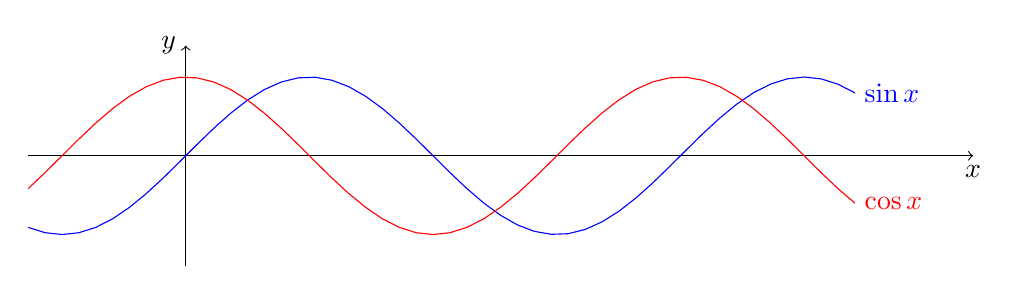
\begin{tikzpicture}
[domain=-2:8.5,samples=50]

  %\draw[very thin,color=lightgray] (-0.1,-1.1) grid (3.9,3.9);
  \draw[->] (-2.0,0) -- (10.0,0) node[below] {$x$};
  \draw[->] (0,-1.4) -- (0,1.4) node[left]  {$y$};

  % \x r means to convert '\x' from degrees to _r_adians:
  \draw[color=blue] plot (\x,{sin(\x r)}) node[right] {$\sin x$};
  \draw[color=red]  plot (\x,{cos(\x r)}) node[right] {$\cos x$};
\end{tikzpicture}
\end{figure}

There are also differential and functional equations for sine and cosine that are reminiscent of the corresponding equations for the exponential function. Sine and cosine satisfy the following system of coupled differential equations:
\begin{equation}
\frac{d}{dx} \sin(x) = \cos(x), \quad
\frac{d}{dx} \cos(x) = -\sin(x)
\end{equation}
and the following system of coupled functional equations which are also known under the name of \emph{addition theorems}:
\begin{equation}
\sin(x+y) = \sin(x) \cos(y) + \cos(x) \sin(y), \qquad
\cos(x+y) = \cos(x) \cos(y) - \sin(x) \sin(y)
\end{equation}
Although the relations are more complicated for sine and cosine than they are for the exponential function, we see that sine and cosine also somehow seem to translate between addition and multiplication and the derivatives are also repetitive. This is not a coincidence. In fact, the pair of sine and cosine are related to the exponential function in the complex domain via the formula:
\begin{equation}
\e^{\i z} = \cos(z) + \i \sin(z)
\end{equation}
for any complex number $z$. 






% https://tikz.dev/tikz-plots

%Yes - we can also plug complex numbers into $\sin, \cos$ and $\exp$. How to evaluate them for complex arguments is completely defined via the series expansions because all of these three series expansions do indeed converge in the entire complex plane.  ...TBC...

% Maybe introduce sin/cos similar to how sinh/cosh were introduced. But here, we have to do:
% sin(z) = e^{i z} - e^{- i z} / (2i)  = Im e^z
% cos(z) = e^{i z} + e^{- i z} / (2)   = Re e^z
% i.e. instead of extracting even and odd part, we extract real and imaginary part
% Oh - but we have to consider e^{i y} for real y, i.e. evaluate exp at the imaginary axis.





% Explain symmetries (oddness, evenness) of sine and cosine and periodicity
% Explain how the terms in these series formulas represent the odd and even terms of the exponetial series with alternating signs


% https://en.wikipedia.org/wiki/Sine_and_cosine
% https://en.wikipedia.org/wiki/List_of_trigonometric_identities

% Explain how the series for cos and sin arise from the series of the exponential function by splitting it inot real and imaginary part




% https://www.youtube.com/watch?v=-PYEguPdwdk
% 27:40
% -The addition theorems:
%    cos(x+y) = ...
%    sin(x+y) = ...
%  can be thought of as being analoguous to the functional equation for the exponential function.
%  But it is more complicated - namely a system of two coupled functional equations.
% -Give also the system of differential equations:  sin' = cos, cos' = -sin'


%---------------------------------------------------------------------------------------------------
\subsubsection{Relations between Exponential, Hyperbolic and Trigonometric Functions}

...TBC...

% https://en.wikipedia.org/wiki/Gudermannian_function


%---------------------------------------------------------------------------------------------------
\subsubsection{Inverse Functions}

\paragraph{Logarithms}
We have seen that the exponential function $f(x) = \e^x$ is injective, i.e. maps different inputs to different outputs. It is not surjective on $\mathbb{R}$ though, because the negative values are never reached by $f$. However, if we restrict its codomain to $\mathbb{R}^+$, i.e. to only those values that are actually reached, then we can define an inverse function $g: \mathbb{R}^+ \rightarrow \mathbb{R}$ of the exponential function $f(x) = \e^x$. We call this function the \emph{natural logarithm} ...TBC...

% See:
% https://www.youtube.com/watch?v=Xv8jkBHknLM
% at: 2:41, 4:52, 5:25, 7:30, 9:15, 15:40, 17:40, 20:55, 23:00

%% ToDo:
% -functional equation
% -derivative (maybe - it's a preview to calc)
% -rules (base-change, etc.)
% -notational ambiguities (log vs ln, lg, ld, lb)


% https://www.youtube.com/watch?v=_LGevgfq4UY
% -sin' = cos works only when we give the argument in radians
% -Conversion of complex numbers from cartesian to polar coordinates: 
%  r = sqrt(x^2 + y^2), cos(t) = x/r -> t = sign(y) * acos(x/r), sin(t) = y/r -> t = asin(y/r)
%  t = atan2(y,x)  -> brauch kein r
% -arkus-funktion, weil sie eine bogenlänge zurückliefert (arkus heißt Bogen)
% -(asin(x))' = 1 / sqrt(1 - x^2)
% -(tanx(x))' = 1 / cos^2(x) = 1 + tan^2(x)
% -(atanx(x))' = 1 / (1 + x^2) 

%---------------------------------------------------------------------------------------------------
\subsubsection{Partial Functions}
In our set-theoretic description, functions were also required to be \emph{left-total} relations. When we drop the left-totality requirement, we arrive at the notion of a \emph{partial function}. For such a partial function from a set $X$ to a set $Y$ we do not require the function value to be defined for any $x \in X$. There may be some $x \in X$ for which $f(x)$ is undefined. In such a case, we may write $f(x) = \, \perp$ and we may indicate missing function values by using a "partial arrow" like so: $f: X \rightharpoonup Y$. The $\perp$ symbol is special symbol that indicates an undefined value. It it sometimes called the \emph{bottom}\footnote{In a different context, namely in geometry and linear algebra, the same symbol $\perp$ is used to indicate that two things are perpendicular. There, we may call it "perp". But here in this context, we use it for "bottom"} element. Consider the function $f(x) = 1/x$. Because division by zero is impossible, we could interpret $f$ as partial function $f: \mathbb{R} \rightharpoonup \mathbb{R}$ and set $f(0) = \, \perp$. Another possibility would be to exclude $0$ from the domain by writing $f: \mathbb{R} \setminus \{ 0 \} \rightarrow \mathbb{R}$. A third possibility would be to define $f(0)$ as any arbitrary value, i.e. define the function conditionally using different definitions in different cases. For example, we could arbitrarily define $f(0) = 0$ and $f(x) = 1/x$ for nonzero $x$. Yet another way to deal with the situation is to consider the function as mapping the real numbers to the so called projectively extended real number line\footnote{In the projectively extended real line we don't distinguish between $+\infty$ and $-\infty$. There, both infinities merge into a single one. This will be explored further in the chapter about algebraic geometry which makes extensive use of such "projective" spaces.}, i.e. $f: \mathbb{R} \rightarrow \mathbb{R} \cup \{ \infty \}$. But this is a topic for a different chapter. The takeaway here is that there are different ways for dealing with problematic input values and one of them is to define the function as a partial function.


%Sometimes though, we may be a bit sloppy with that and nevertheless write $f: \mathbb{R} \rightarrow \mathbb{R}$.

% https://en.wikipedia.org/wiki/Projectively_extended_real_line

%Often, we may be a bit sloppy with that

% https://en.wikipedia.org/wiki/Partial_function
% https://en.wikipedia.org/wiki/Wheel_theory
% https://en.wikipedia.org/wiki/Greatest_element_and_least_element
% https://en.wikipedia.org/wiki/Projectively_extended_real_line
% https://en.wikipedia.org/wiki/Extended_real_number_line


%---------------------------------------------------------------------------------------------------
\subsubsection{Multifunctions}
In the set-theoretic framework, functions are required to be \emph{right-unique} relations. We sometimes need to work with function-like objects that violate this condition. \emph{Multifunctions} are multi valued functions in the sense that for a given input $x$ they produce not a unique output value $y$ but multiple values. For example, consider the equation $x^2 = 4$. It has the two solutions $+2$ and $-2$. \emph{The} square root of $4$ on $\mathbb{R}$ is usually \emph{defined} to be $+2$ - but that's a matter of definition. It would also be viable to define the square root to be multi-valued, i.e. set-valued. Then, instead of giving the solution $2$, it would give the solution $\{2,-2\}$. The output would not be a single number but a whole set of numbers. Allowing the output to be set-valued is one way to view multifunctions. Another approach to view a multifunction is to go back to the set-theoretical definition of a function as a left-total and right-unique relation and just drop the "right-unique" requirement.

% https://en.wikipedia.org/wiki/Multivalued_function
% https://en.wikipedia.org/wiki/Set-valued_function
% https://math.stackexchange.com/questions/3726882/square-root-as-a-multi-valued-function


\paragraph{Complex Roots}
In the real numbers $\mathbb{R}$, when taking the $n$th root for a given real number $x$ and a given positive natural number $n$, we denote the result or root as $y = \sqrt[n]{x}$. It all works out fine when $n$ is odd. In this case, $y = \sqrt[n]{x}$ defines a bona-fide function because the equation $y^n = x$ will always have a unique real-valued solution $y$. For even $n$, however, we run into two problems: for negative $x$, there is no real solution whatsoever and for positive $x$, there are two real solutions. We usually "solve" the problem by saying: okay, for even $n$, the function $\sqrt[n]{x}$ is undefined whenever $x < 0$. That is: we turn $\sqrt[n]{x}$ into a partial function that is defined only for nonnegative inputs $x$. Where the function is defined, i.e. for $x \geq 0$, we pick the nonnegative solution from the two possible solutions by definition. This is an ugly hack. We may get kinda away with it on $\mathbb{R}$ but when we enter the complex plane $\mathbb{C}$, it is not good enough anymore. In $\mathbb{R}$, we would say that $\sqrt[4]{16} = 2$. In $\mathbb{C}$, we would say that $\sqrt[4]{16} = \{2,2\i,-2,-2\i\}$. In general, the $n$th root of any nonzero complex number $z$ will produce a set of $n$ solutions. To write down the set of solutions, i.e. the set of function values $w = \sqrt[n]{z}$, let's express our input number $z$ in polar form as $z = r \e^{i \varphi}$ where $r = |z|, \varphi = \arg(z) = \angle(z)$. Then we can define the solution set $w$ as:
\begin{equation}
 \label{Eq:ComplexRoots}
 w = \{ w_k : k \in \{0,\ldots,n-1\} \}
 \qquad \text{where} \qquad
 w_k = \sqrt[n]{r} \, \exp \left( \frac{\i (\varphi + 2 \pi k) }{n} \right)
\end{equation}
Let's unpack this. The variable $w$ stands for a whole set of solutions, namely the set $w = \{w_0, w_1, \ldots, w_{n-1}\}$. Each of these $w_k$ is a uniquely defined complex number which can be computed by the formula to right of equation (\ref{Eq:ComplexRoots}). The first factor in the formula $\sqrt[n]{r}$ is just an $n$th root of a nonnegative real number, so we have no problems computing it. The result will be again a nonnegative real number. The second factor $\exp \left( \frac{\i (\varphi + 2 \pi k) }{n} \right)$ is a complex exponential function of a purely imaginary argument. That will give us a complex number on the unit circle. Multiplying by such a number yields a pure rotation around the origin - so the second factor gives us a rotation factor. 

\medskip
We can interpret the two factors geometrically as follows: The first factor gives us the radius of the $k$th solution. This radius does not depend on the index $k$, so it will be the same for all $k$. The second factor determines the angle of our $k$th solution. This angle does indeed depend on $k$. The solutions lie all on a circle of radius $\sqrt[n]{r}$ and they are evenly distributed around this circle. The angle of our first solution for $k=0$ is given by $\frac{\varphi}{n}$. The angle difference between two successive solutions is always the same and given by $\frac{2 \pi}{n}$. 

\medskip
I said earlier that we will get $n$ roots when the input $z$ is nonzero. So, what happens at zero? Well, the formulas pose no problems whatsoever but all the computed solutions will coincide because the first factor, the radius, will be zero. In terms of polynomial roots, we can interpret this as a single solution/root at zero with a multiplicity of $n$.

%For $z=0$, we'll get only one solution, namely zero. 

 ...TBC...explain branches, main branch, branch cuts, roots of unity, what happens at $z=0$

% https://en.wikipedia.org/wiki/Nth_root#Complex_roots
% https://de.wikipedia.org/wiki/Wurzel_(Mathematik)#Wurzeln_aus_komplexen_Zahlen

\paragraph{Complex Logarithms}
For logarithms on $\mathbb{C}$, things get even crazier. Due to the periodicity of the complex exponential function, the complex logarithm of any nonzero complex number $z$ is an infinite set. The natural logarithm $w$ of any number $z$ must satisfy $\e^w = z$. Let's write $z$ again as $z = r \e^{\i \varphi}$. Then, the logarithm $w = \log(z)$ can be computed as follows:
\begin{equation}
 \label{Eq:ComplexLogarithm}
 w = \{ w_k : k \in \mathbb{Z}  \}
 \qquad \text{where} \qquad
 w_k = \log(r) + \i (\varphi + 2 \pi k)
\end{equation}
Let's again unpack what the formulas say. This time, the solution set $w$ has infinitely many elements. We get a solution of each $k \in \mathbb{Z}$. The solution with integer index $k$ can be computed via the formula to the right. The first term $\log(r)$ is just the natural logarithm of a positive real number, so no problems here. This will yield the real part of our $k$th solution and that real part actually doesn't even depend on the index $k$, so it will be the same for all $k$. The second term $\i (\varphi + 2 \pi k)$ gives us the imaginary part of our $k$th solution. This part does indeed depend on $k$. 

\medskip
Geometrically, the solutions all line up on a vertical line with real part, i.e. $x$-coordinate, given by $\log(r)$. The imaginary part, i.e. $y$-coordinate, of the solution for $k=0$ is at $\varphi$ and the solutions for all other values of $k$ are spaced apart by multiples of $2 \pi$ in the vertical direction.  

\medskip
Again, we need to pay attention to what happens at $z=0$. In this case, we would have $r = |z| = 0$, so we would need to compute $\log(0)$ for the first term. The logarithm of zero is undefined and that is indeed situation beyond repair\footnote{Maybe one could try something with $-\infty$ for $\Re(w_k)$ but I have no idea if that could work out in a meaningful way. Probably not. ToDo: figure out!}. There is no complex number $w$ that satisfies $\e^w = 0$ because the exponential function always produces nonzero values. So, in light of what we learned about partial functions, the complex logarithm could be defined as a partial multifunction or we just define it as a regular multifunction $f: \mathbb{C} \setminus \{ 0 \} \rightarrow \mathbb{C}$ which is the typical way to do it.

...TBC...explain main branch, principal value

% i.e. the fact that $e^z = e^{z + 2 \pi k \i}$ for any integer $k$, 
% $\log(z)$

% I think, the logarithm is actually a partial multifunction - it's multivalued but undefined for 0


% https://en.wikipedia.org/wiki/Complex_logarithm
% https://en.wikipedia.org/wiki/Argument_(complex_analysis)#Principal_value

%the square-root function on the real numbers. 
% what about fractional roots like the (7/5)th root? ...or in general, how about z^w for any complex exponent w? how about irrational roots

%If you go back to the diagram showing the rela  Fig. ..., 

% -Maybe we can view multifunctions also simply as relations where we relax the condition of being
%  right-unique

\paragraph{Inverse Trigonometric Functions} 
We do not really need to enter the complex plane to appreciate the usefulness of the idea of a multifunction. The concept makes sense already in a purely real context. ...TBC...

% https://en.wikipedia.org/wiki/Inverse_trigonometric_functions





%===================================================================================================
\subsection{Special Functions}

\subsubsection{The Logarithmic Integrals $\li(x)$ and $\Li(x)$}
The \emph{logarithmic integral} functions $\li(x)$ and $\Li(x)$ are defined via an integral as:
\begin{equation}
\label{Eq:LogarithmicIntegral}
 \li(x) = \int_{0}^{x} \frac{1}{\log(t)} \; dt, \qquad
 \Li(x) = \int_{2}^{x} \frac{1}{\log(t)} \; dt
        = \li(x) - \li(2)
\end{equation}
The second variant is called the \emph{offset logarithmic integral} or the \emph{Eulerian logarithmic integral} and is more convenient in number theory, for example. ...TBC...

% https://en.wikipedia.org/wiki/Logarithmic_integral_function
% https://mathworld.wolfram.com/LogarithmicIntegral.html

\subsubsection{The Gamma Function $\Gamma(x)$}
The Gamma function, denoted as $\Gamma(z)$, can be seen as a generalization of the (shifted) factorial function $(n-1)!$ to the whole complex plane. For $\Re(z)>0$ it is usually defined via a parameter integral like so:
\begin{equation}
\Gamma(z) =	\int_{0}^{\infty} t^{z-1} \e^{-t} \, dt 
          = 2 \int_{0}^{\infty} t^{2z-1} \e^{-t^2} \, dt 
          = \int_{0}^{1} (\log(1/t))^{z-1}  \, dt 	
\end{equation}
Some important properties are:
\begin{equation}
\Gamma(n) = (n-1)!, \quad	
\Gamma(z+1) = z \Gamma(z), \quad
\Gamma(\overline{z}) = \overline{\Gamma(z)}, \quad
\Gamma(z) \Gamma(1-z) = \frac{\pi}{\sin(\pi z)}
\end{equation}
The first equation is a statement that $\Gamma$ interpolates the shifted factorial. The second says that the functional equation known from the factorial continues to hold for general complex inputs $z$. The third...TBC...


% Two nice approximations for n!
% https://www.youtube.com/watch?v=PN3qGwyl-dY
%   (1)  sqrt(2 \pi n) (n/e)^n  <  n!  <  e sqrt(n) (n/e)^n
%   (2)  ((n+1)/3)^n  <  n!  <   ((n+1)/2)^n
% Maybe these approximations could be useful in some contexts. The first formula in (1) is 
% Stirling's approximations. It may be useful to know that it is an approximation from below. Maybe
% we can construct a prcatically useful better approximatiosn by somehow averaging an approximation
% from above with one from below? We could experiment with different kinds of (weighted) averages. 
% Or maybe we could somehow constrcut an intermediate approximation. For example, we could use
% ((n+1)/2.5)^n  which is in between  ((n+1)/3)^n  and  ((n+1)/2)^n

% Stirling-Formel (Mathe-Song)
% https://www.youtube.com/watch?v=laJJfH6urrA

%where I have also listed some of its important properties, namely

% https://mathworld.wolfram.com/GammaFunction.html
% https://en.wikipedia.org/wiki/Gamma_function

%https://www.youtube.com/watch?v=R7djflEwPwQ
% gamma, bessel, elliptic integrals



\begin{comment}

-polynomials, rational functions, power series, trig-functions, exp/log, floor/ceil/round, atan2
-maybe explain functions also as unary operators? abs, negation


How to define functions:

done:
-explicitly, e.g. y = x^2
-piecewise (may also be explicit but that's actually an independent question)
-by data (togther with an interpolation rule)
-Dirichlet function: "infinitely piecewise"? "pointwise"? "condition-based"? How about:
 f(x) = numerator, if x rational otherwise 0
-by an algorithm (see fractal functions (Bolzano function) Weitz video "Monster der Analysis")
 -> limit of an infinite recursive process
-power series - this is the usual way to expand definitions of function to e.g. complex 
 numbers, matrices, etc.
-other types of series , example: Weierstrass function - also in "Monster der Analysis"
-series in some domain, analytic continuation where the series diverges, example:
 Riemann Zeta function.
-functional equations, examples: 
 f(x + y) = f(x) * f(y)  ->  f(x) = exp(x)
 f(a x) = b f(x)  ->  f(x) = x^(b/a) or x^(a/b)
 f(x+1) = x * f(x) -> Gamma-function, leads to a definition via an integral
-(parameter) integrals...?
-implicit functions ...maybe something like 
 y + exp(y) = x + sin(x), y - exp(y) = x + sin(x), y - exp(y) = x - sin(x), y + exp(y) = sqrt(x^x)
 is this an example?: https://en.wikipedia.org/wiki/Lambert_W_function
 if not, then maybe it should be considered as yet another way to define a function
 y e^y = x -> g(x,y) = x - y e^y

todo:
-definite or indefinite integral of some given function, examples:
 erf (int of Gauss), jacobi-elliptic (int of 1/sqrt(...))
-as the solution of a given problem (let f(x) be the solution of ..blabla)
-differential equations, examples: Bessel
-integral equation, example: assume that a kernel h(x) is given (for example Gauss-func) and
 some function g(x) is given. We seek f(x) such that g = convolve(f,h). Useful in signal reconstruction (compensate for undesired filtering)
-delay differential? what about something like f(x+1/2) - f(x-1/2) = f'(x) or equivalently
 f(x+1) - f(x) = f'(x + 1/2). Idea: we want a function whose derivative equals the central
 difference approximation of it. "differentio-functional"?
-maybe it makes sense to have a section about equations - what type of equations we see in math...but for some types (e.g. differntial or integral equations), we need some calculus
-what about the Dirac delta function? It's not really a function, though

-Maybe start the section of elementary functions with a list of the simplemost functions in 
 that order: f(x) = 0, f(x) = a, f(x) = x, f(x) = x + a,  f(x) = a x, f(x) = a x + b
 ...maybe f(x) = 1/x or f(x) = a/x can also be on this list of kindergarten-functions
 
For trig functions:
-explain reference angles:
 https://courses.lumenlearning.com/csn-precalculus/chapter/reference-angles/
 they result from the symmetries of sin/cos. 
 sin is odd around 0 + k \pi, and even around \pi / 2  + k \pi and for cos, it's the other
 way around
 
Maybe move the stuff about polynomials and rational functions into a section of its own. 
It's too much for a subsubsection under Functions. Maybe make a section
Elementary Functions:
-Polynomials
 -Add, Multiply, Divide (with remainder), Compose
-Rational Functions
 -Partial Fraction Expansion
Includ these formulas:
https://en.wikipedia.org/wiki/Quartic_function#General_formula_for_roots 
https://en.wikipedia.org/wiki/Quartic_equation#Alternative_methods


https://en.wikipedia.org/wiki/List_of_mathematical_functions
https://en.wikipedia.org/wiki/Dawson_function


https://www.youtube.com/watch?v=Jz8VCv1MIYE
has at 5:29 an example for a function that is everywhere smooth but nowhere analytic

\end{comment}

%Numbers (N,Z,Q,R,C), Polynomials, Rational Functions, Transcendental Functions